\documentclass{article}
\usepackage{float, hyperref}
\usepackage[margin=1in]{geometry}
\usepackage{graphicx}
\usepackage{hyperref}
\usepackage{caption}

\usepackage{Sweave}
\begin{document}
\Sconcordance{concordance:Significance_Overall.tex:Significance_Overall.Rnw:%
1 7 1 1 0 7 1 1 5 2 1 1 19 1 6 5 0 2 1 1 2 1 0 2 2 1 0 1 6 4 0 1 2 3 1 %
1 3 1 0 1 2 1 0 1 2 1 0 1 2 1 0 1 2 1 0 2 2 1 0 2 2 1 0 1 1 1 2 1 0 1 3 %
2 0 1 1 1 2 3 0 1 2 2 1 1 2 5 0 1 2 5 1 1 2 5 0 1 2 5 1 1 2 5 0 1 2 5 1 %
1 2 5 0 1 2 5 1 1 2 5 0 1 2 5 1 1 2 5 0 1 2 4 1}


\author{Lindsay Rutter}
\title{Cluster Analysis of Wasps}

\maketitle

  
\section*{Introduction}


\begin{Schunk}
\begin{Sinput}
> #%%%%%%%%%%%%%%%%%%%%%%%%%%%%%%%%%%%%%%%%%%%%%%%%%%%%%%%%%%%%%%%%%%%%%%%%%%%%%%%%%%%%%%%%%%%
> #%%%%%%%%%%%%%%%%%%%%%%%%%%%%%%%%%%%%%%%%%%%%%%%%%%%%%%%%%%%%%%%%%%%%%%%%%%%%%%%%%%%%%%%%%%%
> ##################################### EXTRA DATA QUALITY####################################
> 
> rm(list=ls())
> load("All_wasp.rda")
> listcond = rep(c("DR","DU","F","NR","NU"),each= 6)
> # 157,691 genes
> y = DGEList(counts=countTable, group=listcond)
> keep <- rowSums(cpm(y)>1) >= 6
> # it seems library sizes are recalculated (y$samples$lib.size = colSums(y$counts))
> y <- y[keep, keep.lib.sizes=FALSE]
> ######################### EXTRA FILTERING AT THIS STEP ########################
> 
> RowSD = function(x) {
+   sqrt(rowSums((x - rowMeans(x))^2)/(dim(x)[2] - 1))
+ }
> yt = y
> yt2 = as.data.frame(yt[[1]])
> y = mutate(yt2, mean = (DR.1+DR.2+DR.3+DR.4+DR.5+DR.6+DU.1+DU.2+DU.3+DU.4+DU.5+DU.6+F.1+F.2+F.3+F.4+F.5+F.6+NR.1+NR.2+NR.3+NR.4+NR.5+NR.6+NU.1+NU.2+NU.3+NU.4+NU.5+NU.6)/ncol(yt2), stdev = RowSD(cbind(DR.1,DR.2,DR.3,DR.4,DR.5,DR.6,DU.1,DU.2,DU.3,DU.4,DU.5,DU.6,F.1,F.2,F.3,F.4,F.5,F.6,NR.1,NR.2,NR.3,NR.4,NR.5,NR.6,NU.1,NU.2,NU.3,NU.4,NU.5,NU.6)))
> rownames(y)=rownames(yt)
> # The first quartile threshold of mean counts across the 12 samples
> q1T = as.numeric(summary(y$mean)["1st Qu."])
> # 24,610 genes
> d2q1 = subset(y,mean>q1T)
> # The first quartile threshold of standard deviation across the 12 samples
> q1Ts = as.numeric(summary(d2q1$stdev)["1st Qu."])
> # 18,458 genes
> d2q1 = subset(d2q1,stdev>q1Ts)
> # 14,355
> filt = subset(y,mean<=q1T|stdev<=q1Ts)
> model = loess(mean ~ stdev, data=d2q1)
> # 11,998 genes
> d2q1 = d2q1[which(sign(model$residuals) == 1),]
> d2q1 = d2q1[,1:(ncol(d2q1)-2)]
> # (filt 14,355 genes)
> filt = filt[,1:(ncol(filt)-2)]
> colnames(filt)=colnames(d2q1)
> # filt (30,670 genes)
> filt = rbind(filt,d2q1[which(sign(model$residuals) == -1),])
> #filts = t(apply(as.matrix(filt), 1, scale))
> #colnames(filts)=colnames(d2q1)
> colnames(filt)=colnames(d2q1)
> y = DGEList(counts=d2q1, group=listcond)
> y = calcNormFactors(y)
\end{Sinput}
\end{Schunk}

\begin{figure}[H]
\centering
\begin{Schunk}
\begin{Sinput}
> ggparcoord(data.frame(y[[1]]), columns=1:ncol(y[[1]]), alphaLines=0, boxplot=TRUE, scale="globalminmax") + coord_flip() + scale_y_log10()
\end{Sinput}
\end{Schunk}
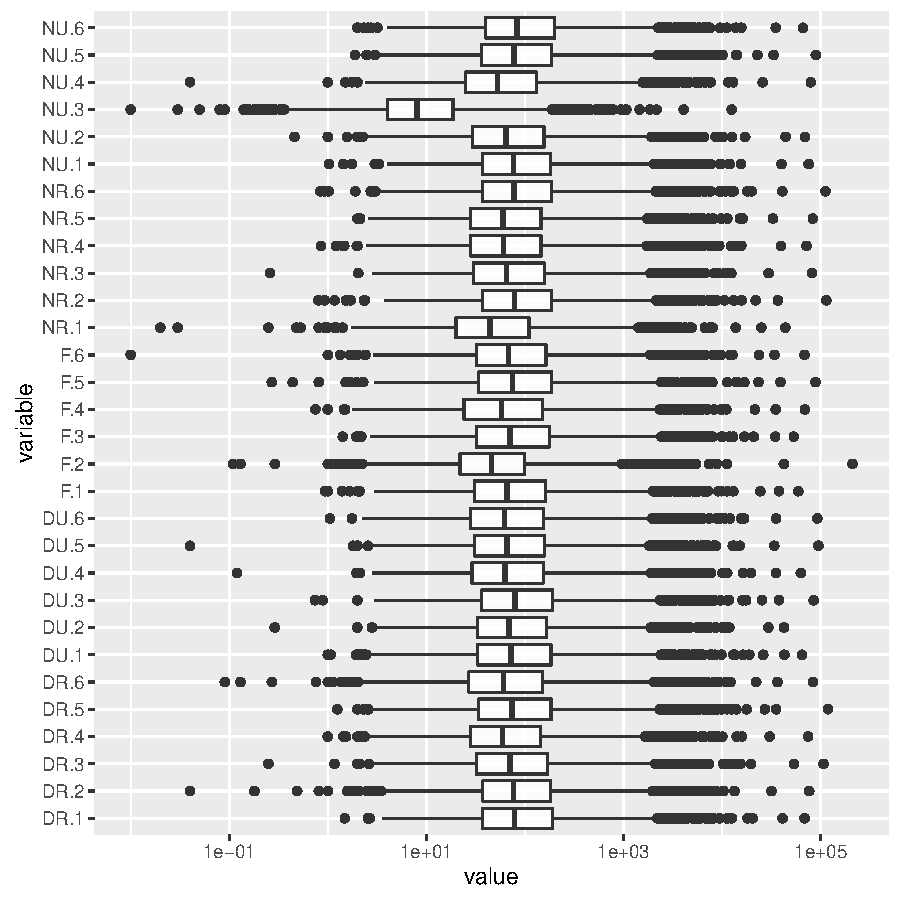
\includegraphics{Significance_Overall-004}
\caption{This is all data filtered on CPM and filtered by Loess, then normalized.}
\label{Boxd2q1}
\end{figure}

\begin{figure}[H]
\centering
\begin{Schunk}
\begin{Sinput}
> ggparcoord(data.frame(y[[1]]), columns=1:6, scale="globalminmax", alphaLines = 0.07)
\end{Sinput}
\end{Schunk}
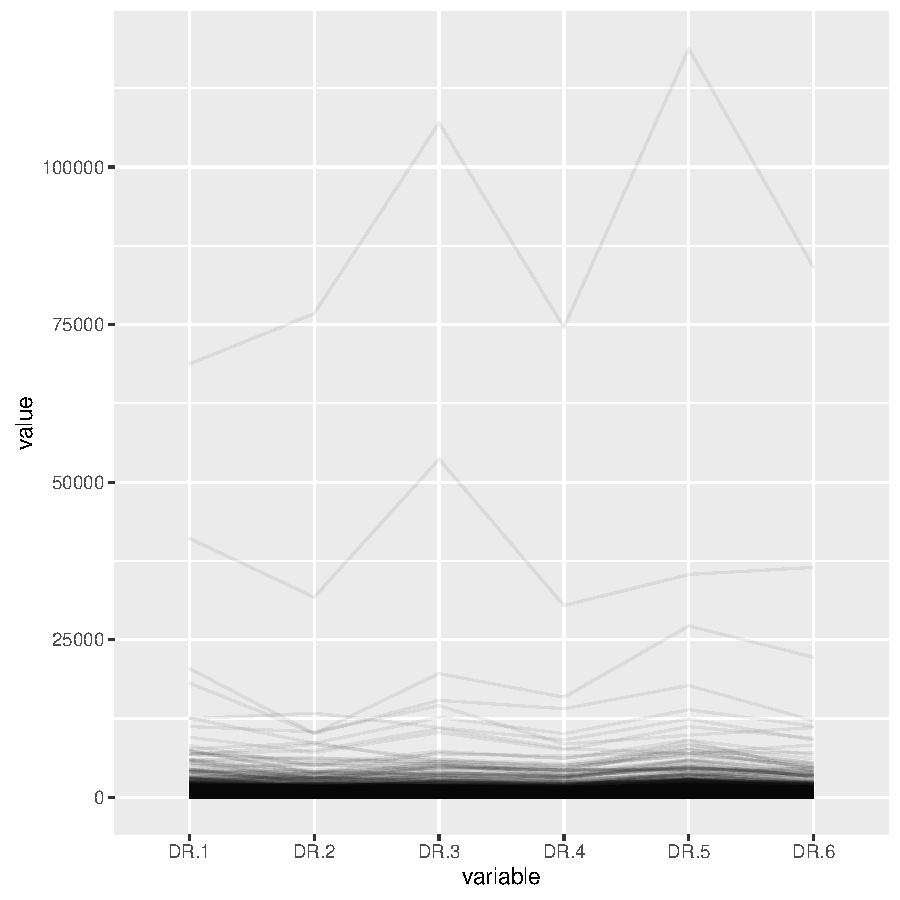
\includegraphics{Significance_Overall-005}
\caption{DR PCP}
\label{Boxd2q1s}
\end{figure}

\begin{figure}[H]
\centering
\begin{Schunk}
\begin{Sinput}
> ggparcoord(data.frame(y[[1]]), columns=7:12, scale="globalminmax", alphaLines = 0.07)
\end{Sinput}
\end{Schunk}
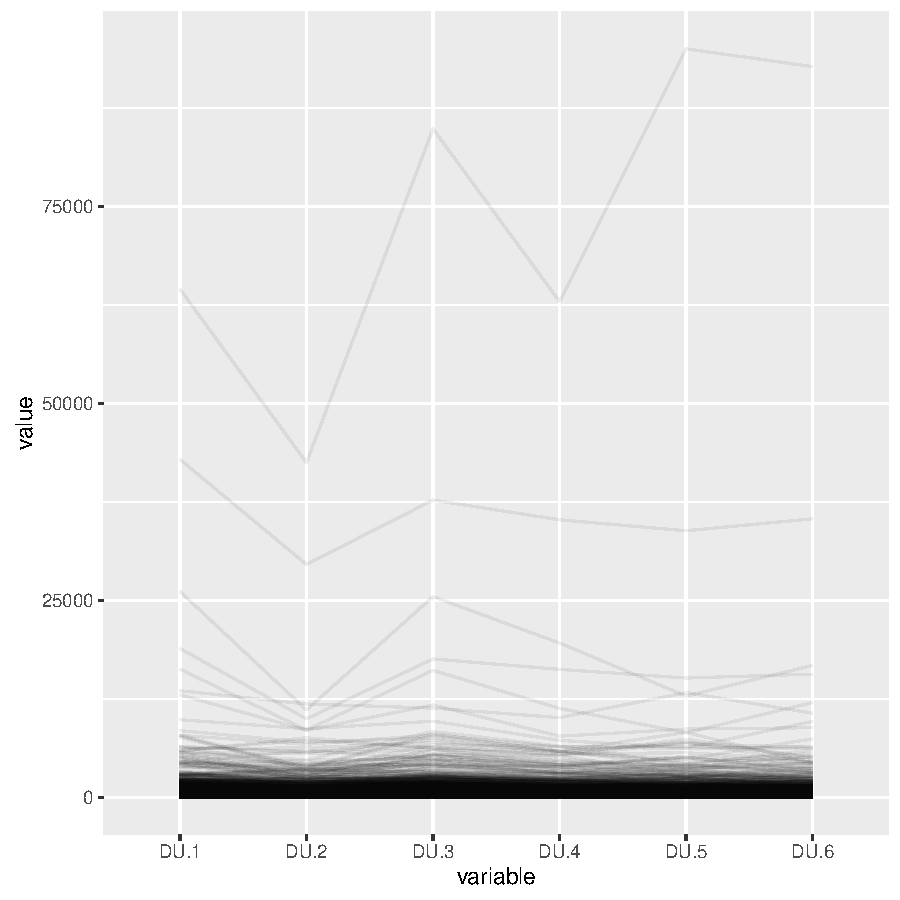
\includegraphics{Significance_Overall-006}
\caption{DU PCP}
\label{Boxd2q1s}
\end{figure}

\begin{figure}[H]
\centering
\begin{Schunk}
\begin{Sinput}
> ggparcoord(data.frame(y[[1]]), columns=13:18, scale="globalminmax", alphaLines = 0.07)
\end{Sinput}
\end{Schunk}
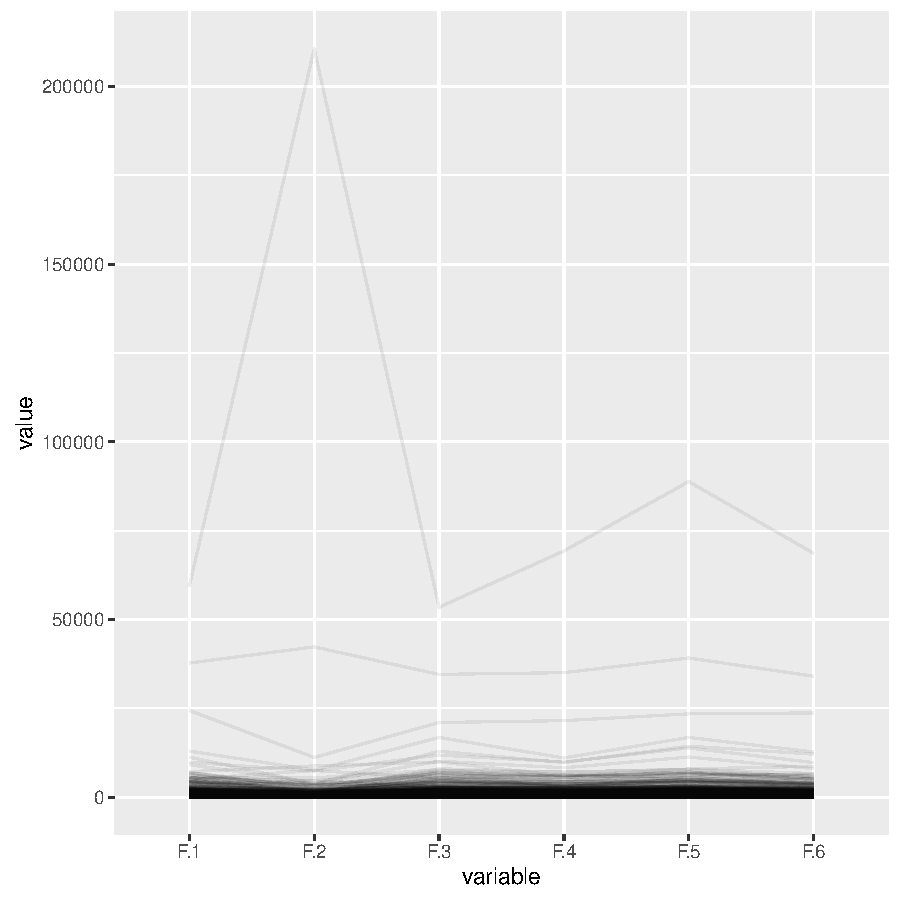
\includegraphics{Significance_Overall-007}
\caption{F PCP}
\label{Boxd2q1s}
\end{figure}

\begin{figure}[H]
\centering
\begin{Schunk}
\begin{Sinput}
> ggparcoord(data.frame(y[[1]]), columns=19:24, scale="globalminmax", alphaLines = 0.07)
\end{Sinput}
\end{Schunk}
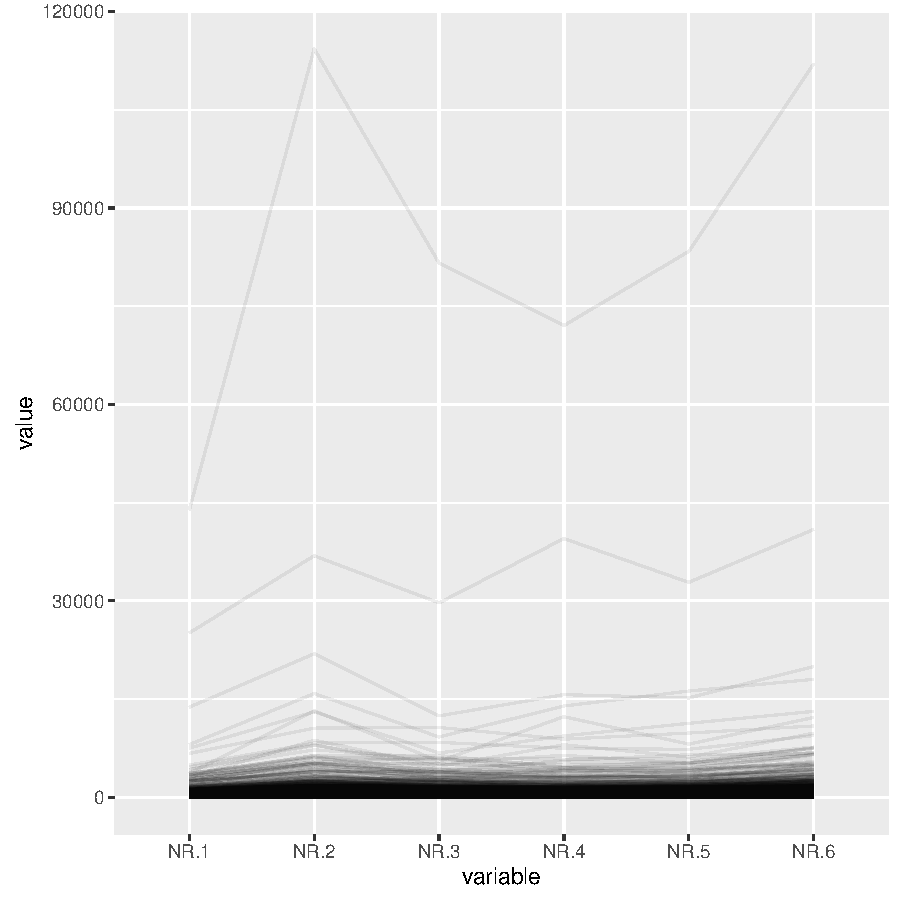
\includegraphics{Significance_Overall-008}
\caption{NR PCP}
\label{Boxd2q1s}
\end{figure}

\begin{figure}[H]
\centering
\begin{Schunk}
\begin{Sinput}
> ggparcoord(data.frame(y[[1]]), columns=25:30, scale="globalminmax", alphaLines = 0.07)
\end{Sinput}
\end{Schunk}
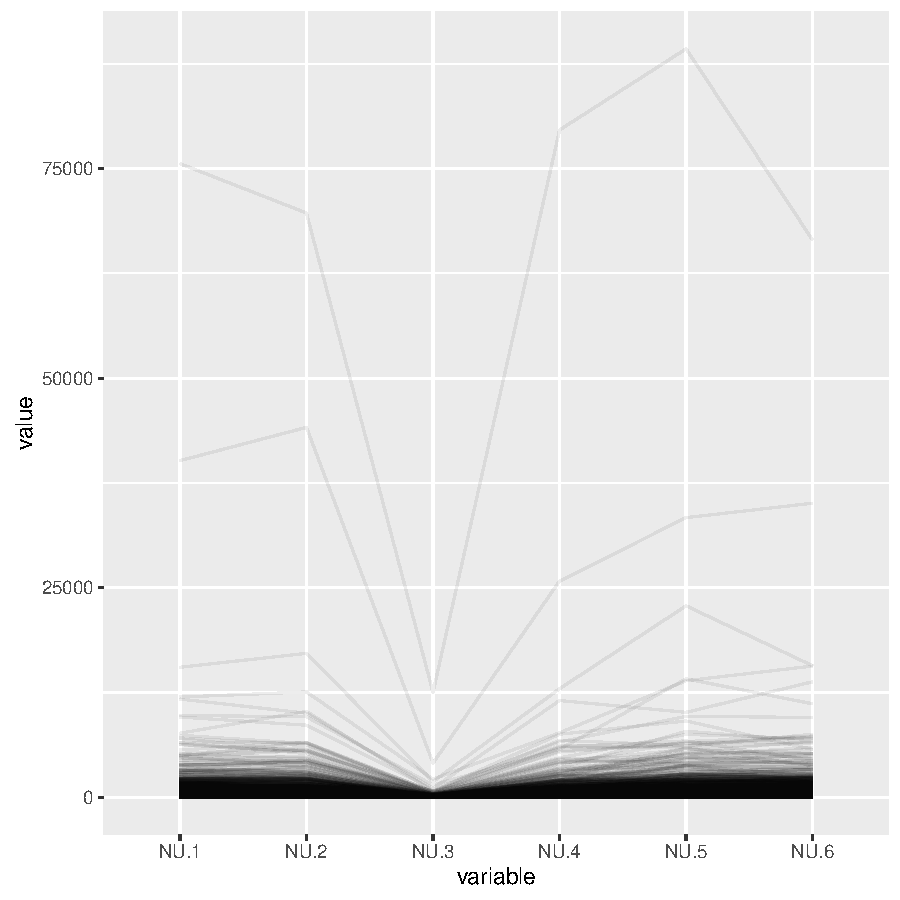
\includegraphics{Significance_Overall-009}
\caption{NU PCP}
\label{Boxd2q1s}
\end{figure}

\end{document}
